\documentclass[1p]{elsarticle_modified}
%\bibliographystyle{elsarticle-num}

%\usepackage[colorlinks]{hyperref}
%\usepackage{abbrmath_seonhwa} %\Abb, \Ascr, \Acal ,\Abf, \Afrak
\usepackage{amsfonts}
\usepackage{amssymb}
\usepackage{amsmath}
\usepackage{amsthm}
\usepackage{scalefnt}
\usepackage{amsbsy}
\usepackage{kotex}
\usepackage{caption}
\usepackage{subfig}
\usepackage{color}
\usepackage{graphicx}
\usepackage{xcolor} %% white, black, red, green, blue, cyan, magenta, yellow
\usepackage{float}
\usepackage{setspace}
\usepackage{hyperref}

\usepackage{tikz}
\usetikzlibrary{arrows}

\usepackage{multirow}
\usepackage{array} % fixed length table
\usepackage{hhline}

%%%%%%%%%%%%%%%%%%%%%
\makeatletter
\renewcommand*\env@matrix[1][\arraystretch]{%
	\edef\arraystretch{#1}%
	\hskip -\arraycolsep
	\let\@ifnextchar\new@ifnextchar
	\array{*\c@MaxMatrixCols c}}
\makeatother %https://tex.stackexchange.com/questions/14071/how-can-i-increase-the-line-spacing-in-a-matrix
%%%%%%%%%%%%%%%

\usepackage[normalem]{ulem}

\newcommand{\msout}[1]{\ifmmode\text{\sout{\ensuremath{#1}}}\else\sout{#1}\fi}
%SOURCE: \msout is \stkout macro in https://tex.stackexchange.com/questions/20609/strikeout-in-math-mode

\newcommand{\cancel}[1]{
	\ifmmode
	{\color{red}\msout{#1}}
	\else
	{\color{red}\sout{#1}}
	\fi
}

\newcommand{\add}[1]{
	{\color{blue}\uwave{#1}}
}

\newcommand{\replace}[2]{
	\ifmmode
	{\color{red}\msout{#1}}{\color{blue}\uwave{#2}}
	\else
	{\color{red}\sout{#1}}{\color{blue}\uwave{#2}}
	\fi
}

\newcommand{\Sol}{\mathcal{S}} %segment
\newcommand{\D}{D} %diagram
\newcommand{\A}{\mathcal{A}} %arc


%%%%%%%%%%%%%%%%%%%%%%%%%%%%%5 test

\def\sl{\operatorname{\textup{SL}}(2,\Cbb)}
\def\psl{\operatorname{\textup{PSL}}(2,\Cbb)}
\def\quan{\mkern 1mu \triangleright \mkern 1mu}

\theoremstyle{definition}
\newtheorem{thm}{Theorem}[section]
\newtheorem{prop}[thm]{Proposition}
\newtheorem{lem}[thm]{Lemma}
\newtheorem{ques}[thm]{Question}
\newtheorem{cor}[thm]{Corollary}
\newtheorem{defn}[thm]{Definition}
\newtheorem{exam}[thm]{Example}
\newtheorem{rmk}[thm]{Remark}
\newtheorem{alg}[thm]{Algorithm}

\newcommand{\I}{\sqrt{-1}}
\begin{document}

%\begin{frontmatter}
%
%\title{Boundary parabolic representations of knots up to 8 crossings}
%
%%% Group authors per affiliation:
%\author{Yunhi Cho} 
%\address{Department of Mathematics, University of Seoul, Seoul, Korea}
%\ead{yhcho@uos.ac.kr}
%
%
%\author{Seonhwa Kim} %\fnref{s_kim}}
%\address{Center for Geometry and Physics, Institute for Basic Science, Pohang, 37673, Korea}
%\ead{ryeona17@ibs.re.kr}
%
%\author{Hyuk Kim}
%\address{Department of Mathematical Sciences, Seoul National University, Seoul 08826, Korea}
%\ead{hyukkim@snu.ac.kr}
%
%\author{Seokbeom Yoon}
%\address{Department of Mathematical Sciences, Seoul National University, Seoul, 08826,  Korea}
%\ead{sbyoon15@snu.ac.kr}
%
%\begin{abstract}
%We find all boundary parabolic representation of knots up to 8 crossings.
%
%\end{abstract}
%\begin{keyword}
%    \MSC[2010] 57M25 
%\end{keyword}
%
%\end{frontmatter}

%\linenumbers
%\tableofcontents
%
\newcommand\colored[1]{\textcolor{white}{\rule[-0.35ex]{0.8em}{1.4ex}}\kern-0.8em\color{red} #1}%
%\newcommand\colored[1]{\textcolor{white}{ #1}\kern-2.17ex	\textcolor{white}{ #1}\kern-1.81ex	\textcolor{white}{ #1}\kern-2.15ex\color{red}#1	}

{\Large $\underline{12a_{0174}~(K12a_{0174})}$}

\setlength{\tabcolsep}{10pt}
\renewcommand{\arraystretch}{1.6}
\vspace{1cm}\begin{tabular}{m{100pt}>{\centering\arraybackslash}m{274pt}}
\multirow{5}{120pt}{
	\centering
	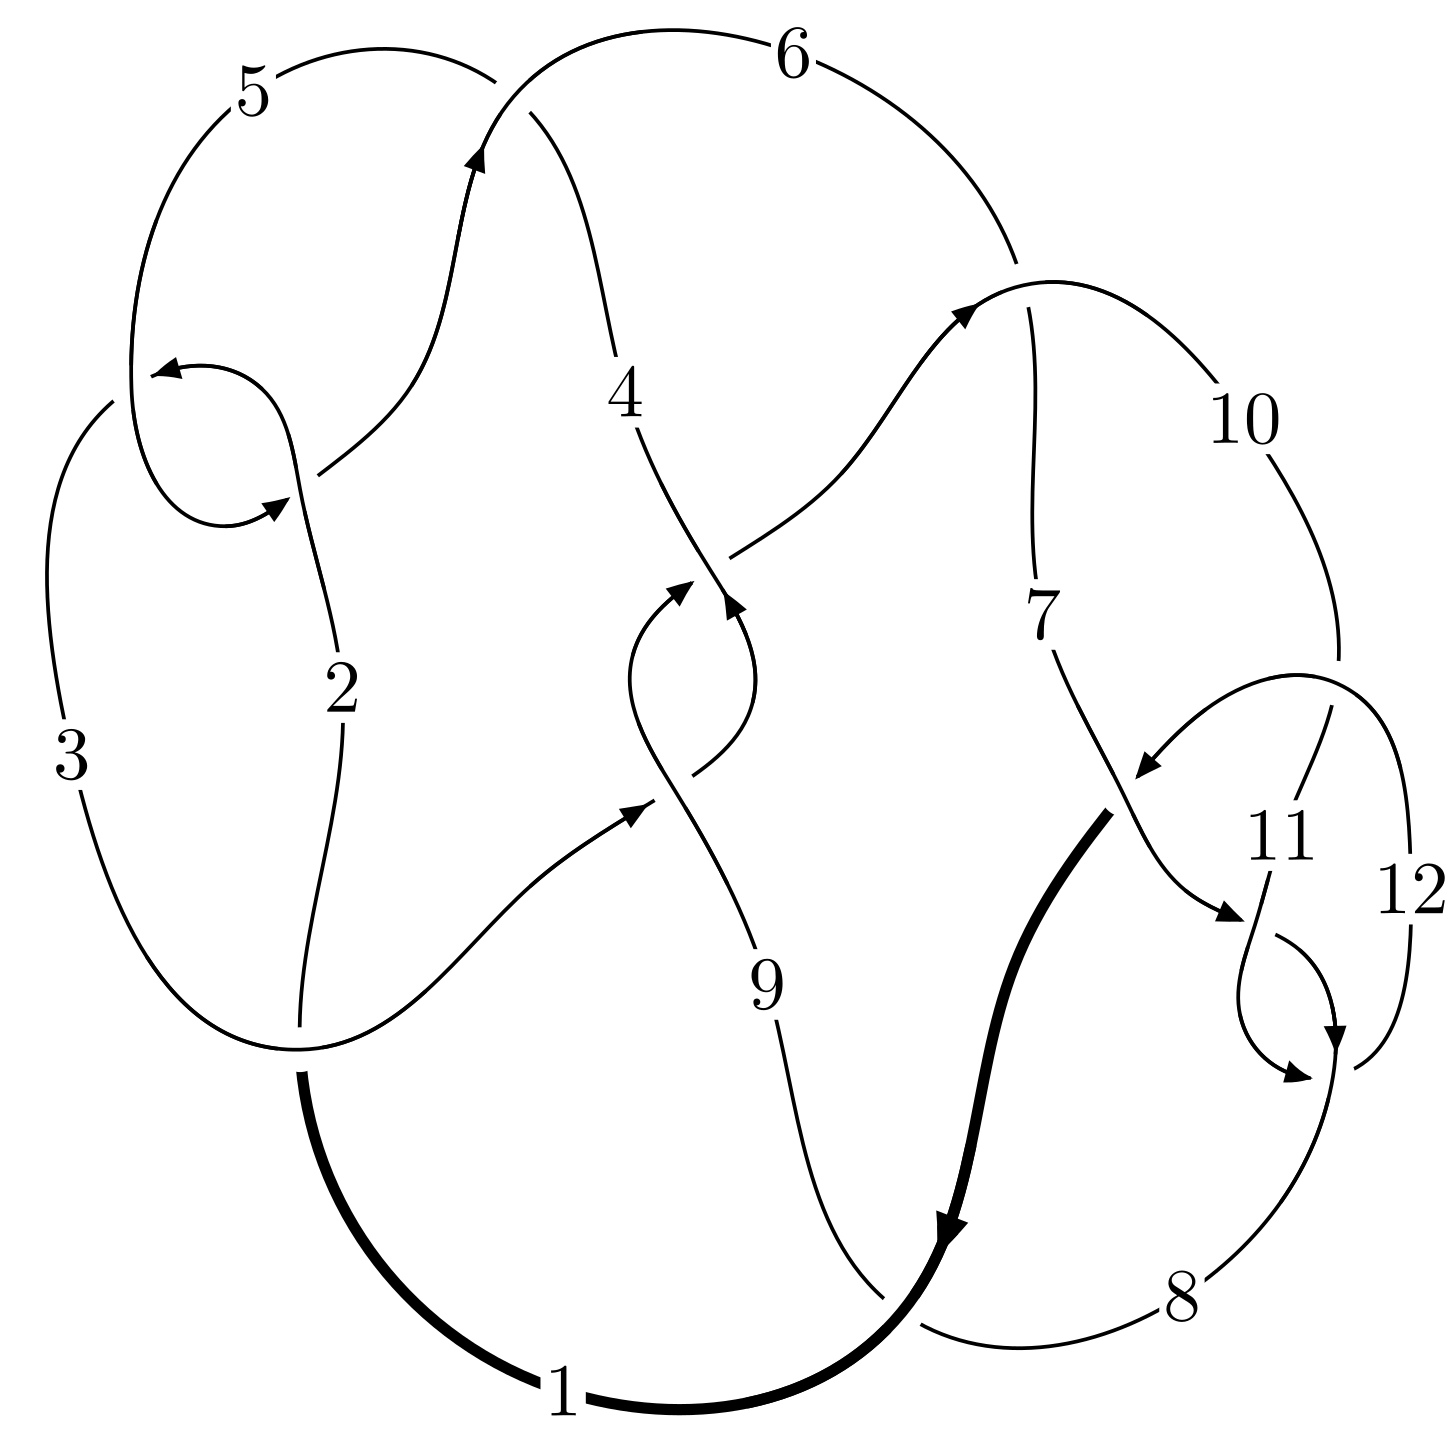
\includegraphics[width=112pt]{../../../GIT/diagram.site/Diagrams/png/975_12a_0174.png}\\
\ \ \ A knot diagram\footnotemark}&
\allowdisplaybreaks
\textbf{Linearized knot diagam} \\
\cline{2-2}
 &
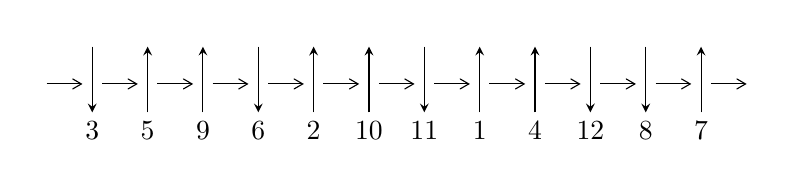
\begin{tikzpicture}[x=20pt, y=17pt]
	% nodes
	\node (C0) at (0, 0) {};
	\node (C1) at (1, 0) {};
	\node (C1U) at (1, +1) {};
	\node (C1D) at (1, -1) {3};

	\node (C2) at (2, 0) {};
	\node (C2U) at (2, +1) {};
	\node (C2D) at (2, -1) {5};

	\node (C3) at (3, 0) {};
	\node (C3U) at (3, +1) {};
	\node (C3D) at (3, -1) {9};

	\node (C4) at (4, 0) {};
	\node (C4U) at (4, +1) {};
	\node (C4D) at (4, -1) {6};

	\node (C5) at (5, 0) {};
	\node (C5U) at (5, +1) {};
	\node (C5D) at (5, -1) {2};

	\node (C6) at (6, 0) {};
	\node (C6U) at (6, +1) {};
	\node (C6D) at (6, -1) {10};

	\node (C7) at (7, 0) {};
	\node (C7U) at (7, +1) {};
	\node (C7D) at (7, -1) {11};

	\node (C8) at (8, 0) {};
	\node (C8U) at (8, +1) {};
	\node (C8D) at (8, -1) {1};

	\node (C9) at (9, 0) {};
	\node (C9U) at (9, +1) {};
	\node (C9D) at (9, -1) {4};

	\node (C10) at (10, 0) {};
	\node (C10U) at (10, +1) {};
	\node (C10D) at (10, -1) {12};

	\node (C11) at (11, 0) {};
	\node (C11U) at (11, +1) {};
	\node (C11D) at (11, -1) {8};

	\node (C12) at (12, 0) {};
	\node (C12U) at (12, +1) {};
	\node (C12D) at (12, -1) {7};
	\node (C13) at (13, 0) {};

	% arrows
	\draw[->,>={angle 60}]
	(C0) edge (C1) (C1) edge (C2) (C2) edge (C3) (C3) edge (C4) (C4) edge (C5) (C5) edge (C6) (C6) edge (C7) (C7) edge (C8) (C8) edge (C9) (C9) edge (C10) (C10) edge (C11) (C11) edge (C12) (C12) edge (C13) ;	\draw[->,>=stealth]
	(C1U) edge (C1D) (C2D) edge (C2U) (C3D) edge (C3U) (C4U) edge (C4D) (C5D) edge (C5U) (C6D) edge (C6U) (C7U) edge (C7D) (C8D) edge (C8U) (C9D) edge (C9U) (C10U) edge (C10D) (C11U) edge (C11D) (C12D) edge (C12U) ;
	\end{tikzpicture} \\
\hhline{~~} \\& 
\textbf{Solving Sequence} \\ \cline{2-2} 
 &
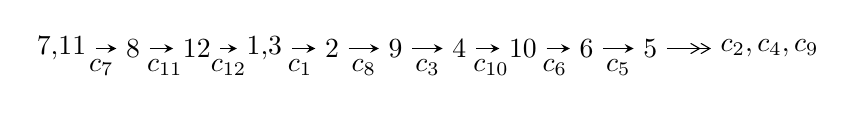
\begin{tikzpicture}[x=23pt, y=7pt]
	% node
	\node (A0) at (-1/8, 0) {7,11};
	\node (A1) at (1, 0) {8};
	\node (A2) at (2, 0) {12};
	\node (A3) at (49/16, 0) {1,3};
	\node (A4) at (33/8, 0) {2};
	\node (A5) at (41/8, 0) {9};
	\node (A6) at (49/8, 0) {4};
	\node (A7) at (57/8, 0) {10};
	\node (A8) at (65/8, 0) {6};
	\node (A9) at (73/8, 0) {5};
	\node (C1) at (1/2, -1) {$c_{7}$};
	\node (C2) at (3/2, -1) {$c_{11}$};
	\node (C3) at (5/2, -1) {$c_{12}$};
	\node (C4) at (29/8, -1) {$c_{1}$};
	\node (C5) at (37/8, -1) {$c_{8}$};
	\node (C6) at (45/8, -1) {$c_{3}$};
	\node (C7) at (53/8, -1) {$c_{10}$};
	\node (C8) at (61/8, -1) {$c_{6}$};
	\node (C9) at (69/8, -1) {$c_{5}$};
	\node (A10) at (11, 0) {$c_{2},c_{4},c_{9}$};

	% edge
	\draw[->,>=stealth]	
	(A0) edge (A1) (A1) edge (A2) (A2) edge (A3) (A3) edge (A4) (A4) edge (A5) (A5) edge (A6) (A6) edge (A7) (A7) edge (A8) (A8) edge (A9) ;
	\draw[->>,>={angle 60}]	
	(A9) edge (A10);
\end{tikzpicture} \\ 

\end{tabular} \\

\footnotetext{
The image of knot diagram is generated by the software ``\textbf{Draw programme}" developed by Andrew Bartholomew(\url{http://www.layer8.co.uk/maths/draw/index.htm\#Running-draw}), where we modified some parts for our purpose(\url{https://github.com/CATsTAILs/LinksPainter}).
}\phantom \\ \newline 
\centering \textbf{Ideals for irreducible components\footnotemark of $X_{\text{par}}$} 
 
\begin{align*}
I^u_{1}&=\langle 
2 u^{94}-6 u^{93}+\cdots+2 b-2,\;-2 u^{94}+2 u^{93}+\cdots+2 a-1,\;u^{95}-3 u^{94}+\cdots-2 u+1\rangle \\
I^u_{2}&=\langle 
- u^5 a+2 u^3 a-2 a u+b,\;- u^4 a- u^5- u^4+u^2 a+u^3+a^2+a u+u^2+u,\;u^6+u^5- u^4-2 u^3+u+1\rangle \\
\\
\end{align*}
\raggedright * 2 irreducible components of $\dim_{\mathbb{C}}=0$, with total 107 representations.\\
\footnotetext{All coefficients of polynomials are rational numbers. But the coefficients are sometimes approximated in decimal forms when there is not enough margin.}
\newpage
\renewcommand{\arraystretch}{1}
\centering \section*{I. $I^u_{1}= \langle 2 u^{94}-6 u^{93}+\cdots+2 b-2,\;-2 u^{94}+2 u^{93}+\cdots+2 a-1,\;u^{95}-3 u^{94}+\cdots-2 u+1 \rangle$}
\flushleft \textbf{(i) Arc colorings}\\
\begin{tabular}{m{7pt} m{180pt} m{7pt} m{180pt} }
\flushright $a_{7}=$&$\begin{pmatrix}1\\0\end{pmatrix}$ \\
\flushright $a_{11}=$&$\begin{pmatrix}0\\u\end{pmatrix}$ \\
\flushright $a_{8}=$&$\begin{pmatrix}1\\u^2\end{pmatrix}$ \\
\flushright $a_{12}=$&$\begin{pmatrix}- u\\- u^3+u\end{pmatrix}$ \\
\flushright $a_{1}=$&$\begin{pmatrix}- u^3\\- u^3+u\end{pmatrix}$ \\
\flushright $a_{3}=$&$\begin{pmatrix}u^{94}- u^{93}+\cdots+2 u+\frac{1}{2}\\- u^{94}+3 u^{93}+\cdots-\frac{5}{2} u+1\end{pmatrix}$ \\
\flushright $a_{2}=$&$\begin{pmatrix}- u^{94}+2 u^{93}+\cdots+u+\frac{3}{2}\\\frac{1}{2} u^{91}-\frac{1}{2} u^{90}+\cdots- u^2+\frac{1}{2} u\end{pmatrix}$ \\
\flushright $a_{9}=$&$\begin{pmatrix}u^8- u^6+u^4+1\\u^8-2 u^6+2 u^4\end{pmatrix}$ \\
\flushright $a_{4}=$&$\begin{pmatrix}u^{94}-6 u^{93}+\cdots+3 u-\frac{5}{2}\\-5 u^{94}+6 u^{93}+\cdots+3 u^2-\frac{7}{2} u\end{pmatrix}$ \\
\flushright $a_{10}=$&$\begin{pmatrix}u^3\\u^5- u^3+u\end{pmatrix}$ \\
\flushright $a_{6}=$&$\begin{pmatrix}u^8- u^6+u^4+1\\u^{10}-2 u^8+3 u^6-2 u^4+u^2\end{pmatrix}$ \\
\flushright $a_{5}=$&$\begin{pmatrix}\frac{3}{2} u^{94}-\frac{11}{2} u^{93}+\cdots+4 u-\frac{3}{2}\\-\frac{7}{2} u^{94}+\frac{9}{2} u^{93}+\cdots+\frac{5}{2} u^2-\frac{5}{2} u\end{pmatrix}$\\&\end{tabular}
\flushleft \textbf{(ii) Obstruction class $= -1$}\\~\\
\flushleft \textbf{(iii) Cusp Shapes $= 4 u^{94}-\frac{27}{2} u^{93}+\cdots+\frac{13}{2} u-2$}\\~\\
\newpage\renewcommand{\arraystretch}{1}
\flushleft \textbf{(iv) u-Polynomials at the component}\newline \\
\begin{tabular}{m{50pt}|m{274pt}}
Crossings & \hspace{64pt}u-Polynomials at each crossing \\
\hline $$\begin{aligned}c_{1},c_{4}\end{aligned}$$&$\begin{aligned}
&u^{95}+29 u^{94}+\cdots-12 u-1
\end{aligned}$\\
\hline $$\begin{aligned}c_{2},c_{5}\end{aligned}$$&$\begin{aligned}
&u^{95}+7 u^{94}+\cdots-4 u-1
\end{aligned}$\\
\hline $$\begin{aligned}c_{3},c_{9}\end{aligned}$$&$\begin{aligned}
&u^{95}+u^{94}+\cdots-12288 u-4096
\end{aligned}$\\
\hline $$\begin{aligned}c_{6},c_{8}\end{aligned}$$&$\begin{aligned}
&u^{95}-3 u^{94}+\cdots+4216 u-1201
\end{aligned}$\\
\hline $$\begin{aligned}c_{7},c_{11}\end{aligned}$$&$\begin{aligned}
&u^{95}+3 u^{94}+\cdots-2 u-1
\end{aligned}$\\
\hline $$\begin{aligned}c_{10}\end{aligned}$$&$\begin{aligned}
&u^{95}+43 u^{94}+\cdots+8 u+1
\end{aligned}$\\
\hline $$\begin{aligned}c_{12}\end{aligned}$$&$\begin{aligned}
&u^{95}+9 u^{94}+\cdots+6 u+1
\end{aligned}$\\
\hline
\end{tabular}\\~\\
\newpage\renewcommand{\arraystretch}{1}
\flushleft \textbf{(v) Riley Polynomials at the component}\newline \\
\begin{tabular}{m{50pt}|m{274pt}}
Crossings & \hspace{64pt}Riley Polynomials at each crossing \\
\hline $$\begin{aligned}c_{1},c_{4}\end{aligned}$$&$\begin{aligned}
&y^{95}+81 y^{94}+\cdots-492 y-1
\end{aligned}$\\
\hline $$\begin{aligned}c_{2},c_{5}\end{aligned}$$&$\begin{aligned}
&y^{95}+29 y^{94}+\cdots-12 y-1
\end{aligned}$\\
\hline $$\begin{aligned}c_{3},c_{9}\end{aligned}$$&$\begin{aligned}
&y^{95}-65 y^{94}+\cdots+184549376 y-16777216
\end{aligned}$\\
\hline $$\begin{aligned}c_{6},c_{8}\end{aligned}$$&$\begin{aligned}
&y^{95}-83 y^{94}+\cdots+13537528 y-1442401
\end{aligned}$\\
\hline $$\begin{aligned}c_{7},c_{11}\end{aligned}$$&$\begin{aligned}
&y^{95}-43 y^{94}+\cdots+8 y-1
\end{aligned}$\\
\hline $$\begin{aligned}c_{10}\end{aligned}$$&$\begin{aligned}
&y^{95}+21 y^{94}+\cdots-44 y-1
\end{aligned}$\\
\hline $$\begin{aligned}c_{12}\end{aligned}$$&$\begin{aligned}
&y^{95}+y^{94}+\cdots+76 y-1
\end{aligned}$\\
\hline
\end{tabular}\\~\\
\newpage\flushleft \textbf{(vi) Complex Volumes and Cusp Shapes}
$$\begin{array}{c|c|c}  
\text{Solutions to }I^u_{1}& \I (\text{vol} + \sqrt{-1}CS) & \text{Cusp shape}\\
 \hline 
\begin{aligned}
u &= -0.780961 + 0.613854 I \\
a &= -1.148870 - 0.337111 I \\
b &= \phantom{-}0.164002 + 1.387420 I\end{aligned}
 & \phantom{-}6.51601 - 0.63092 I & \phantom{-0.000000 } 0 \\ \hline\begin{aligned}
u &= -0.780961 - 0.613854 I \\
a &= -1.148870 + 0.337111 I \\
b &= \phantom{-}0.164002 - 1.387420 I\end{aligned}
 & \phantom{-}6.51601 + 0.63092 I & \phantom{-0.000000 } 0 \\ \hline\begin{aligned}
u &= -0.814626 + 0.609563 I \\
a &= \phantom{-}1.35420 + 0.79384 I \\
b &= \phantom{-}0.471342 - 1.314330 I\end{aligned}
 & \phantom{-}6.41936 + 5.44116 I & \phantom{-0.000000 } 0 \\ \hline\begin{aligned}
u &= -0.814626 - 0.609563 I \\
a &= \phantom{-}1.35420 - 0.79384 I \\
b &= \phantom{-}0.471342 + 1.314330 I\end{aligned}
 & \phantom{-}6.41936 - 5.44116 I & \phantom{-0.000000 } 0 \\ \hline\begin{aligned}
u &= \phantom{-}0.962721 + 0.330637 I \\
a &= \phantom{-}0.362055 + 0.865330 I \\
b &= -0.390291 + 0.463584 I\end{aligned}
 & -1.64642 - 1.19817 I & \phantom{-0.000000 } 0 \\ \hline\begin{aligned}
u &= \phantom{-}0.962721 - 0.330637 I \\
a &= \phantom{-}0.362055 - 0.865330 I \\
b &= -0.390291 - 0.463584 I\end{aligned}
 & -1.64642 + 1.19817 I & \phantom{-0.000000 } 0 \\ \hline\begin{aligned}
u &= \phantom{-}0.550887 + 0.774748 I \\
a &= \phantom{-}0.203078 - 0.527598 I \\
b &= \phantom{-}0.91385 - 2.47044 I\end{aligned}
 & \phantom{-}11.5214 - 8.2023 I & \phantom{-0.000000 } 0 \\ \hline\begin{aligned}
u &= \phantom{-}0.550887 - 0.774748 I \\
a &= \phantom{-}0.203078 + 0.527598 I \\
b &= \phantom{-}0.91385 + 2.47044 I\end{aligned}
 & \phantom{-}11.5214 + 8.2023 I & \phantom{-0.000000 } 0 \\ \hline\begin{aligned}
u &= \phantom{-}0.538994 + 0.781645 I \\
a &= -0.413072 + 0.514846 I \\
b &= -1.21805 + 1.93499 I\end{aligned}
 & \phantom{-}12.33230 - 1.87951 I & \phantom{-0.000000 } 0 \\ \hline\begin{aligned}
u &= \phantom{-}0.538994 - 0.781645 I \\
a &= -0.413072 - 0.514846 I \\
b &= -1.21805 - 1.93499 I\end{aligned}
 & \phantom{-}12.33230 + 1.87951 I & \phantom{-0.000000 } 0\\
 \hline 
 \end{array}$$\newpage$$\begin{array}{c|c|c}  
\text{Solutions to }I^u_{1}& \I (\text{vol} + \sqrt{-1}CS) & \text{Cusp shape}\\
 \hline 
\begin{aligned}
u &= -1.049250 + 0.090947 I \\
a &= -1.13294 - 1.38229 I \\
b &= -1.130640 - 0.708429 I\end{aligned}
 & -1.41613 - 3.48168 I & \phantom{-0.000000 } 0 \\ \hline\begin{aligned}
u &= -1.049250 - 0.090947 I \\
a &= -1.13294 + 1.38229 I \\
b &= -1.130640 + 0.708429 I\end{aligned}
 & -1.41613 + 3.48168 I & \phantom{-0.000000 } 0 \\ \hline\begin{aligned}
u &= \phantom{-}1.057200 + 0.026608 I \\
a &= \phantom{-}0.53847 - 3.81847 I \\
b &= \phantom{-}0.32449 - 1.51301 I\end{aligned}
 & \phantom{-}1.39128 + 2.84660 I & \phantom{-0.000000 } 0 \\ \hline\begin{aligned}
u &= \phantom{-}1.057200 - 0.026608 I \\
a &= \phantom{-}0.53847 + 3.81847 I \\
b &= \phantom{-}0.32449 + 1.51301 I\end{aligned}
 & \phantom{-}1.39128 - 2.84660 I & \phantom{-0.000000 } 0 \\ \hline\begin{aligned}
u &= \phantom{-}1.038650 + 0.212196 I \\
a &= \phantom{-}1.54257 - 0.91022 I \\
b &= \phantom{-}0.952348 + 0.006395 I\end{aligned}
 & -3.09968 - 0.14692 I & \phantom{-0.000000 } 0 \\ \hline\begin{aligned}
u &= \phantom{-}1.038650 - 0.212196 I \\
a &= \phantom{-}1.54257 + 0.91022 I \\
b &= \phantom{-}0.952348 - 0.006395 I\end{aligned}
 & -3.09968 + 0.14692 I & \phantom{-0.000000 } 0 \\ \hline\begin{aligned}
u &= -1.06742\phantom{ +0.000000I} \\
a &= -0.00525876\phantom{ +0.000000I} \\
b &= \phantom{-}0.484339\phantom{ +0.000000I}\end{aligned}
 & \phantom{-}2.20266\phantom{ +0.000000I} & \phantom{-0.000000 } 0 \\ \hline\begin{aligned}
u &= \phantom{-}0.442792 + 0.809663 I \\
a &= -0.447657 - 0.371359 I \\
b &= -0.11488 - 2.77795 I\end{aligned}
 & \phantom{-}11.78680 + 5.10800 I & \phantom{-0.000000 } 0 \\ \hline\begin{aligned}
u &= \phantom{-}0.442792 - 0.809663 I \\
a &= -0.447657 + 0.371359 I \\
b &= -0.11488 + 2.77795 I\end{aligned}
 & \phantom{-}11.78680 - 5.10800 I & \phantom{-0.000000 } 0 \\ \hline\begin{aligned}
u &= -0.998749 + 0.411686 I \\
a &= -0.51601 - 2.07092 I \\
b &= -0.89051 - 1.32331 I\end{aligned}
 & -1.81484 - 0.05574 I & \phantom{-0.000000 } 0\\
 \hline 
 \end{array}$$\newpage$$\begin{array}{c|c|c}  
\text{Solutions to }I^u_{1}& \I (\text{vol} + \sqrt{-1}CS) & \text{Cusp shape}\\
 \hline 
\begin{aligned}
u &= -0.998749 - 0.411686 I \\
a &= -0.51601 + 2.07092 I \\
b &= -0.89051 + 1.32331 I\end{aligned}
 & -1.81484 + 0.05574 I & \phantom{-0.000000 } 0 \\ \hline\begin{aligned}
u &= \phantom{-}0.431435 + 0.809966 I \\
a &= \phantom{-}0.262891 + 0.408976 I \\
b &= -0.33236 + 3.10094 I\end{aligned}
 & \phantom{-}10.8466 + 11.3857 I & \phantom{-0.000000 } 0 \\ \hline\begin{aligned}
u &= \phantom{-}0.431435 - 0.809966 I \\
a &= \phantom{-}0.262891 - 0.408976 I \\
b &= -0.33236 - 3.10094 I\end{aligned}
 & \phantom{-}10.8466 - 11.3857 I & \phantom{-0.000000 } 0 \\ \hline\begin{aligned}
u &= \phantom{-}0.481177 + 0.776347 I \\
a &= -0.635172 + 0.078226 I \\
b &= -0.154742 - 0.414216 I\end{aligned}
 & \phantom{-}7.59709 + 1.51037 I & \phantom{-0.000000 } 0 \\ \hline\begin{aligned}
u &= \phantom{-}0.481177 - 0.776347 I \\
a &= -0.635172 - 0.078226 I \\
b &= -0.154742 + 0.414216 I\end{aligned}
 & \phantom{-}7.59709 - 1.51037 I & \phantom{-0.000000 } 0 \\ \hline\begin{aligned}
u &= -0.488387 + 0.768831 I \\
a &= \phantom{-}0.226129 - 0.739384 I \\
b &= -0.52679 - 3.19996 I\end{aligned}
 & \phantom{-}6.78240 + 1.47720 I & \phantom{-0.000000 } 0 \\ \hline\begin{aligned}
u &= -0.488387 - 0.768831 I \\
a &= \phantom{-}0.226129 + 0.739384 I \\
b &= -0.52679 + 3.19996 I\end{aligned}
 & \phantom{-}6.78240 - 1.47720 I & \phantom{-0.000000 } 0 \\ \hline\begin{aligned}
u &= \phantom{-}0.985538 + 0.468332 I \\
a &= \phantom{-}1.71416 + 1.11430 I \\
b &= -0.53775 + 1.45196 I\end{aligned}
 & -0.41801 - 1.39796 I & \phantom{-0.000000 } 0 \\ \hline\begin{aligned}
u &= \phantom{-}0.985538 - 0.468332 I \\
a &= \phantom{-}1.71416 - 1.11430 I \\
b &= -0.53775 - 1.45196 I\end{aligned}
 & -0.41801 + 1.39796 I & \phantom{-0.000000 } 0 \\ \hline\begin{aligned}
u &= -0.470750 + 0.775433 I \\
a &= \phantom{-}0.007864 + 0.757463 I \\
b &= \phantom{-}1.22123 + 3.04799 I\end{aligned}
 & \phantom{-}6.68359 - 4.44968 I & \phantom{-0.000000 } 0\\
 \hline 
 \end{array}$$\newpage$$\begin{array}{c|c|c}  
\text{Solutions to }I^u_{1}& \I (\text{vol} + \sqrt{-1}CS) & \text{Cusp shape}\\
 \hline 
\begin{aligned}
u &= -0.470750 - 0.775433 I \\
a &= \phantom{-}0.007864 - 0.757463 I \\
b &= \phantom{-}1.22123 - 3.04799 I\end{aligned}
 & \phantom{-}6.68359 + 4.44968 I & \phantom{-0.000000 } 0 \\ \hline\begin{aligned}
u &= \phantom{-}0.498994 + 0.747728 I \\
a &= \phantom{-}0.553295 - 0.061468 I \\
b &= -0.488696 - 0.759297 I\end{aligned}
 & \phantom{-}3.92549 - 2.45104 I & \phantom{-0.000000 } 0 \\ \hline\begin{aligned}
u &= \phantom{-}0.498994 - 0.747728 I \\
a &= \phantom{-}0.553295 + 0.061468 I \\
b &= -0.488696 + 0.759297 I\end{aligned}
 & \phantom{-}3.92549 + 2.45104 I & \phantom{-0.000000 } 0 \\ \hline\begin{aligned}
u &= \phantom{-}0.450266 + 0.769200 I \\
a &= \phantom{-}0.484149 - 0.086895 I \\
b &= -0.85386 + 1.26850 I\end{aligned}
 & \phantom{-}3.65208 + 5.26825 I & \phantom{-}5.67264 - 4.34315 I \\ \hline\begin{aligned}
u &= \phantom{-}0.450266 - 0.769200 I \\
a &= \phantom{-}0.484149 + 0.086895 I \\
b &= -0.85386 - 1.26850 I\end{aligned}
 & \phantom{-}3.65208 - 5.26825 I & \phantom{-}5.67264 + 4.34315 I \\ \hline\begin{aligned}
u &= -0.997603 + 0.486225 I \\
a &= \phantom{-}0.07933 + 1.71375 I \\
b &= \phantom{-}0.850725 + 0.977718 I\end{aligned}
 & -0.26339 + 4.20614 I & \phantom{-0.000000 } 0 \\ \hline\begin{aligned}
u &= -0.997603 - 0.486225 I \\
a &= \phantom{-}0.07933 - 1.71375 I \\
b &= \phantom{-}0.850725 - 0.977718 I\end{aligned}
 & -0.26339 - 4.20614 I & \phantom{-0.000000 } 0 \\ \hline\begin{aligned}
u &= -0.818001 + 0.283222 I \\
a &= -1.22395 + 0.95854 I \\
b &= -0.838364 + 0.628083 I\end{aligned}
 & -0.91580 + 2.96787 I & \phantom{-}5.16431 - 4.85868 I \\ \hline\begin{aligned}
u &= -0.818001 - 0.283222 I \\
a &= -1.22395 - 0.95854 I \\
b &= -0.838364 - 0.628083 I\end{aligned}
 & -0.91580 - 2.96787 I & \phantom{-}5.16431 + 4.85868 I \\ \hline\begin{aligned}
u &= -1.133080 + 0.079025 I \\
a &= -0.74599 + 3.05335 I \\
b &= \phantom{-}0.12767 + 1.70298 I\end{aligned}
 & \phantom{-}6.36459 - 3.00517 I & \phantom{-0.000000 } 0\\
 \hline 
 \end{array}$$\newpage$$\begin{array}{c|c|c}  
\text{Solutions to }I^u_{1}& \I (\text{vol} + \sqrt{-1}CS) & \text{Cusp shape}\\
 \hline 
\begin{aligned}
u &= -1.133080 - 0.079025 I \\
a &= -0.74599 - 3.05335 I \\
b &= \phantom{-}0.12767 - 1.70298 I\end{aligned}
 & \phantom{-}6.36459 + 3.00517 I & \phantom{-0.000000 } 0 \\ \hline\begin{aligned}
u &= \phantom{-}1.033340 + 0.475771 I \\
a &= -2.20424 - 0.41049 I \\
b &= \phantom{-}0.01972 - 1.63353 I\end{aligned}
 & -1.30770 - 6.29698 I & \phantom{-0.000000 } 0 \\ \hline\begin{aligned}
u &= \phantom{-}1.033340 - 0.475771 I \\
a &= -2.20424 + 0.41049 I \\
b &= \phantom{-}0.01972 + 1.63353 I\end{aligned}
 & -1.30770 + 6.29698 I & \phantom{-0.000000 } 0 \\ \hline\begin{aligned}
u &= \phantom{-}1.068430 + 0.396628 I \\
a &= -0.731444 - 0.056111 I \\
b &= -0.051532 - 0.930237 I\end{aligned}
 & -4.58435 - 1.29164 I & \phantom{-0.000000 } 0 \\ \hline\begin{aligned}
u &= \phantom{-}1.068430 - 0.396628 I \\
a &= -0.731444 + 0.056111 I \\
b &= -0.051532 + 0.930237 I\end{aligned}
 & -4.58435 + 1.29164 I & \phantom{-0.000000 } 0 \\ \hline\begin{aligned}
u &= -1.136250 + 0.096416 I \\
a &= \phantom{-}0.24065 - 3.64517 I \\
b &= -0.42912 - 2.02773 I\end{aligned}
 & \phantom{-}5.49121 - 9.18730 I & \phantom{-0.000000 } 0 \\ \hline\begin{aligned}
u &= -1.136250 - 0.096416 I \\
a &= \phantom{-}0.24065 + 3.64517 I \\
b &= -0.42912 + 2.02773 I\end{aligned}
 & \phantom{-}5.49121 + 9.18730 I & \phantom{-0.000000 } 0 \\ \hline\begin{aligned}
u &= \phantom{-}1.118070 + 0.307627 I \\
a &= \phantom{-}0.89147 + 1.34016 I \\
b &= \phantom{-}0.446385 + 1.300890 I\end{aligned}
 & \phantom{-}0.16831 - 2.74248 I & \phantom{-0.000000 } 0 \\ \hline\begin{aligned}
u &= \phantom{-}1.118070 - 0.307627 I \\
a &= \phantom{-}0.89147 - 1.34016 I \\
b &= \phantom{-}0.446385 - 1.300890 I\end{aligned}
 & \phantom{-}0.16831 + 2.74248 I & \phantom{-0.000000 } 0 \\ \hline\begin{aligned}
u &= -1.074940 + 0.455048 I \\
a &= -0.331036 - 0.869702 I \\
b &= -0.983402 - 0.770520 I\end{aligned}
 & -4.19048 + 5.73083 I & \phantom{-0.000000 } 0\\
 \hline 
 \end{array}$$\newpage$$\begin{array}{c|c|c}  
\text{Solutions to }I^u_{1}& \I (\text{vol} + \sqrt{-1}CS) & \text{Cusp shape}\\
 \hline 
\begin{aligned}
u &= -1.074940 - 0.455048 I \\
a &= -0.331036 + 0.869702 I \\
b &= -0.983402 + 0.770520 I\end{aligned}
 & -4.19048 - 5.73083 I & \phantom{-0.000000 } 0 \\ \hline\begin{aligned}
u &= \phantom{-}1.122510 + 0.332451 I \\
a &= -0.269407 - 1.226360 I \\
b &= -0.122905 - 1.274200 I\end{aligned}
 & -0.10202 + 2.84328 I & \phantom{-0.000000 } 0 \\ \hline\begin{aligned}
u &= \phantom{-}1.122510 - 0.332451 I \\
a &= -0.269407 + 1.226360 I \\
b &= -0.122905 + 1.274200 I\end{aligned}
 & -0.10202 - 2.84328 I & \phantom{-0.000000 } 0 \\ \hline\begin{aligned}
u &= -0.405906 + 0.713088 I \\
a &= \phantom{-}0.0772709 + 0.1123500 I \\
b &= \phantom{-}1.131810 + 0.566237 I\end{aligned}
 & \phantom{-}1.26600 - 1.90136 I & \phantom{-}2.51207 - 0.74357 I \\ \hline\begin{aligned}
u &= -0.405906 - 0.713088 I \\
a &= \phantom{-}0.0772709 - 0.1123500 I \\
b &= \phantom{-}1.131810 - 0.566237 I\end{aligned}
 & \phantom{-}1.26600 + 1.90136 I & \phantom{-}2.51207 + 0.74357 I \\ \hline\begin{aligned}
u &= -0.489486 + 0.653058 I \\
a &= \phantom{-}0.219391 - 0.026142 I \\
b &= \phantom{-}0.604620 - 0.877826 I\end{aligned}
 & \phantom{-}1.71463 - 0.14968 I & \phantom{-}4.78717 + 1.52967 I \\ \hline\begin{aligned}
u &= -0.489486 - 0.653058 I \\
a &= \phantom{-}0.219391 + 0.026142 I \\
b &= \phantom{-}0.604620 + 0.877826 I\end{aligned}
 & \phantom{-}1.71463 + 0.14968 I & \phantom{-}4.78717 - 1.52967 I \\ \hline\begin{aligned}
u &= -1.048610 + 0.559029 I \\
a &= -0.84830 + 1.23363 I \\
b &= \phantom{-}0.344607 + 1.144680 I\end{aligned}
 & \phantom{-}0.05936 + 4.88677 I & \phantom{-0.000000 } 0 \\ \hline\begin{aligned}
u &= -1.048610 - 0.559029 I \\
a &= -0.84830 - 1.23363 I \\
b &= \phantom{-}0.344607 - 1.144680 I\end{aligned}
 & \phantom{-}0.05936 - 4.88677 I & \phantom{-0.000000 } 0 \\ \hline\begin{aligned}
u &= \phantom{-}1.037050 + 0.640450 I \\
a &= \phantom{-}3.43025 + 0.11156 I \\
b &= \phantom{-}1.40816 + 2.01666 I\end{aligned}
 & \phantom{-}10.07100 + 2.86446 I & \phantom{-0.000000 } 0\\
 \hline 
 \end{array}$$\newpage$$\begin{array}{c|c|c}  
\text{Solutions to }I^u_{1}& \I (\text{vol} + \sqrt{-1}CS) & \text{Cusp shape}\\
 \hline 
\begin{aligned}
u &= \phantom{-}1.037050 - 0.640450 I \\
a &= \phantom{-}3.43025 - 0.11156 I \\
b &= \phantom{-}1.40816 - 2.01666 I\end{aligned}
 & \phantom{-}10.07100 - 2.86446 I & \phantom{-0.000000 } 0 \\ \hline\begin{aligned}
u &= \phantom{-}1.059720 + 0.608371 I \\
a &= \phantom{-}0.861944 + 0.972153 I \\
b &= -0.415084 + 0.511149 I\end{aligned}
 & \phantom{-}2.25792 - 2.70432 I & \phantom{-0.000000 } 0 \\ \hline\begin{aligned}
u &= \phantom{-}1.059720 - 0.608371 I \\
a &= \phantom{-}0.861944 - 0.972153 I \\
b &= -0.415084 - 0.511149 I\end{aligned}
 & \phantom{-}2.25792 + 2.70432 I & \phantom{-0.000000 } 0 \\ \hline\begin{aligned}
u &= \phantom{-}1.046590 + 0.640226 I \\
a &= -3.02435 + 0.44398 I \\
b &= -1.60073 - 1.41737 I\end{aligned}
 & \phantom{-}10.81700 - 3.47625 I & \phantom{-0.000000 } 0 \\ \hline\begin{aligned}
u &= \phantom{-}1.046590 - 0.640226 I \\
a &= -3.02435 - 0.44398 I \\
b &= -1.60073 + 1.41737 I\end{aligned}
 & \phantom{-}10.81700 + 3.47625 I & \phantom{-0.000000 } 0 \\ \hline\begin{aligned}
u &= -1.123850 + 0.492704 I \\
a &= \phantom{-}1.055900 - 0.745592 I \\
b &= -0.567989 - 0.875408 I\end{aligned}
 & \phantom{-}0.96122 + 10.56030 I & \phantom{-0.000000 } 0 \\ \hline\begin{aligned}
u &= -1.123850 - 0.492704 I \\
a &= \phantom{-}1.055900 + 0.745592 I \\
b &= -0.567989 + 0.875408 I\end{aligned}
 & \phantom{-}0.96122 - 10.56030 I & \phantom{-0.000000 } 0 \\ \hline\begin{aligned}
u &= -1.117800 + 0.509792 I \\
a &= -0.91098 + 1.32408 I \\
b &= \phantom{-}0.752832 + 1.006100 I\end{aligned}
 & \phantom{-}1.50574 + 4.89986 I & \phantom{-0.000000 } 0 \\ \hline\begin{aligned}
u &= -1.117800 - 0.509792 I \\
a &= -0.91098 - 1.32408 I \\
b &= \phantom{-}0.752832 - 1.006100 I\end{aligned}
 & \phantom{-}1.50574 - 4.89986 I & \phantom{-0.000000 } 0 \\ \hline\begin{aligned}
u &= -1.089020 + 0.573261 I \\
a &= \phantom{-}1.59858 + 1.01418 I \\
b &= \phantom{-}1.36667 - 0.50084 I\end{aligned}
 & -0.73386 + 6.83458 I & \phantom{-0.000000 } 0\\
 \hline 
 \end{array}$$\newpage$$\begin{array}{c|c|c}  
\text{Solutions to }I^u_{1}& \I (\text{vol} + \sqrt{-1}CS) & \text{Cusp shape}\\
 \hline 
\begin{aligned}
u &= -1.089020 - 0.573261 I \\
a &= \phantom{-}1.59858 - 1.01418 I \\
b &= \phantom{-}1.36667 + 0.50084 I\end{aligned}
 & -0.73386 - 6.83458 I & \phantom{-0.000000 } 0 \\ \hline\begin{aligned}
u &= -1.070370 + 0.616569 I \\
a &= -4.10787 + 1.29996 I \\
b &= -1.29406 + 3.14806 I\end{aligned}
 & \phantom{-}5.04940 + 3.76135 I & \phantom{-0.000000 } 0 \\ \hline\begin{aligned}
u &= -1.070370 - 0.616569 I \\
a &= -4.10787 - 1.29996 I \\
b &= -1.29406 - 3.14806 I\end{aligned}
 & \phantom{-}5.04940 - 3.76135 I & \phantom{-0.000000 } 0 \\ \hline\begin{aligned}
u &= \phantom{-}1.075990 + 0.618091 I \\
a &= \phantom{-}0.204895 + 0.417350 I \\
b &= -0.052818 + 0.761747 I\end{aligned}
 & \phantom{-}5.82498 - 6.77346 I & \phantom{-0.000000 } 0 \\ \hline\begin{aligned}
u &= \phantom{-}1.075990 - 0.618091 I \\
a &= \phantom{-}0.204895 - 0.417350 I \\
b &= -0.052818 - 0.761747 I\end{aligned}
 & \phantom{-}5.82498 + 6.77346 I & \phantom{-0.000000 } 0 \\ \hline\begin{aligned}
u &= -1.080650 + 0.614563 I \\
a &= \phantom{-}4.41582 - 0.48798 I \\
b &= \phantom{-}1.93659 - 2.88567 I\end{aligned}
 & \phantom{-}4.86780 + 9.69724 I & \phantom{-0.000000 } 0 \\ \hline\begin{aligned}
u &= -1.080650 - 0.614563 I \\
a &= \phantom{-}4.41582 + 0.48798 I \\
b &= \phantom{-}1.93659 + 2.88567 I\end{aligned}
 & \phantom{-}4.86780 - 9.69724 I & \phantom{-0.000000 } 0 \\ \hline\begin{aligned}
u &= \phantom{-}1.087940 + 0.606131 I \\
a &= -1.89689 + 0.29335 I \\
b &= -1.06745 - 1.47271 I\end{aligned}
 & \phantom{-}1.75821 - 10.46800 I & \phantom{-0.000000 } 0 \\ \hline\begin{aligned}
u &= \phantom{-}1.087940 - 0.606131 I \\
a &= -1.89689 - 0.29335 I \\
b &= -1.06745 + 1.47271 I\end{aligned}
 & \phantom{-}1.75821 + 10.46800 I & \phantom{-0.000000 } 0 \\ \hline\begin{aligned}
u &= \phantom{-}1.103320 + 0.620150 I \\
a &= \phantom{-}3.00445 + 1.91427 I \\
b &= \phantom{-}0.35053 + 3.02366 I\end{aligned}
 & \phantom{-}9.8130 - 10.4617 I & \phantom{-0.000000 } 0\\
 \hline 
 \end{array}$$\newpage$$\begin{array}{c|c|c}  
\text{Solutions to }I^u_{1}& \I (\text{vol} + \sqrt{-1}CS) & \text{Cusp shape}\\
 \hline 
\begin{aligned}
u &= \phantom{-}1.103320 - 0.620150 I \\
a &= \phantom{-}3.00445 - 1.91427 I \\
b &= \phantom{-}0.35053 - 3.02366 I\end{aligned}
 & \phantom{-}9.8130 + 10.4617 I & \phantom{-0.000000 } 0 \\ \hline\begin{aligned}
u &= \phantom{-}1.107970 + 0.616328 I \\
a &= -3.72207 - 1.65268 I \\
b &= -0.81689 - 3.27015 I\end{aligned}
 & \phantom{-}8.8261 - 16.7248 I & \phantom{-0.000000 } 0 \\ \hline\begin{aligned}
u &= \phantom{-}1.107970 - 0.616328 I \\
a &= -3.72207 + 1.65268 I \\
b &= -0.81689 + 3.27015 I\end{aligned}
 & \phantom{-}8.8261 + 16.7248 I & \phantom{-0.000000 } 0 \\ \hline\begin{aligned}
u &= -0.217141 + 0.694895 I \\
a &= -0.757905 + 0.260323 I \\
b &= \phantom{-}0.452422 - 0.998289 I\end{aligned}
 & \phantom{-}4.06957 - 0.36434 I & \phantom{-}7.64440 + 0.20889 I \\ \hline\begin{aligned}
u &= -0.217141 - 0.694895 I \\
a &= -0.757905 - 0.260323 I \\
b &= \phantom{-}0.452422 + 0.998289 I\end{aligned}
 & \phantom{-}4.06957 + 0.36434 I & \phantom{-}7.64440 - 0.20889 I \\ \hline\begin{aligned}
u &= -0.175942 + 0.692243 I \\
a &= \phantom{-}0.961313 - 0.565831 I \\
b &= -0.145143 + 0.854305 I\end{aligned}
 & \phantom{-}3.65758 - 6.12809 I & \phantom{-}6.30632 + 5.77573 I \\ \hline\begin{aligned}
u &= -0.175942 - 0.692243 I \\
a &= \phantom{-}0.961313 + 0.565831 I \\
b &= -0.145143 - 0.854305 I\end{aligned}
 & \phantom{-}3.65758 + 6.12809 I & \phantom{-}6.30632 - 5.77573 I \\ \hline\begin{aligned}
u &= \phantom{-}0.563051 + 0.342434 I \\
a &= \phantom{-}0.21207 + 1.94850 I \\
b &= -0.586216 - 0.752758 I\end{aligned}
 & \phantom{-}0.82985 - 2.31768 I & \phantom{-}3.86321 + 5.04546 I \\ \hline\begin{aligned}
u &= \phantom{-}0.563051 - 0.342434 I \\
a &= \phantom{-}0.21207 - 1.94850 I \\
b &= -0.586216 + 0.752758 I\end{aligned}
 & \phantom{-}0.82985 + 2.31768 I & \phantom{-}3.86321 - 5.04546 I \\ \hline\begin{aligned}
u &= -0.474614 + 0.424865 I \\
a &= \phantom{-}0.471420 + 0.106327 I \\
b &= \phantom{-}0.710860 - 0.278059 I\end{aligned}
 & \phantom{-}1.164430 - 0.256982 I & \phantom{-}9.18842 + 0.97858 I\\
 \hline 
 \end{array}$$\newpage$$\begin{array}{c|c|c}  
\text{Solutions to }I^u_{1}& \I (\text{vol} + \sqrt{-1}CS) & \text{Cusp shape}\\
 \hline 
\begin{aligned}
u &= -0.474614 - 0.424865 I \\
a &= \phantom{-}0.471420 - 0.106327 I \\
b &= \phantom{-}0.710860 + 0.278059 I\end{aligned}
 & \phantom{-}1.164430 + 0.256982 I & \phantom{-}9.18842 - 0.97858 I \\ \hline\begin{aligned}
u &= -0.093168 + 0.511687 I \\
a &= -0.032938 - 1.288750 I \\
b &= -0.489285 + 0.324549 I\end{aligned}
 & -1.69450 - 1.94976 I & -0.97114 + 4.55157 I \\ \hline\begin{aligned}
u &= -0.093168 - 0.511687 I \\
a &= -0.032938 + 1.288750 I \\
b &= -0.489285 - 0.324549 I\end{aligned}
 & -1.69450 + 1.94976 I & -0.97114 - 4.55157 I \\ \hline\begin{aligned}
u &= \phantom{-}0.320233 + 0.371519 I \\
a &= -0.36987 - 2.03603 I \\
b &= -0.193491 + 0.947554 I\end{aligned}
 & \phantom{-}0.53986 + 2.49744 I & \phantom{-}1.77366 - 1.90679 I \\ \hline\begin{aligned}
u &= \phantom{-}0.320233 - 0.371519 I \\
a &= -0.36987 + 2.03603 I \\
b &= -0.193491 - 0.947554 I\end{aligned}
 & \phantom{-}0.53986 - 2.49744 I & \phantom{-}1.77366 + 1.90679 I\\
 \hline 
 \end{array}$$\newpage\newpage\renewcommand{\arraystretch}{1}
\centering \section*{II. $I^u_{2}= \langle - u^5 a+2 u^3 a-2 a u+b,\;- u^4 a- u^5- u^4+u^2 a+u^3+a^2+a u+u^2+u,\;u^6+u^5- u^4-2 u^3+u+1 \rangle$}
\flushleft \textbf{(i) Arc colorings}\\
\begin{tabular}{m{7pt} m{180pt} m{7pt} m{180pt} }
\flushright $a_{7}=$&$\begin{pmatrix}1\\0\end{pmatrix}$ \\
\flushright $a_{11}=$&$\begin{pmatrix}0\\u\end{pmatrix}$ \\
\flushright $a_{8}=$&$\begin{pmatrix}1\\u^2\end{pmatrix}$ \\
\flushright $a_{12}=$&$\begin{pmatrix}- u\\- u^3+u\end{pmatrix}$ \\
\flushright $a_{1}=$&$\begin{pmatrix}- u^3\\- u^3+u\end{pmatrix}$ \\
\flushright $a_{3}=$&$\begin{pmatrix}a\\u^5 a-2 u^3 a+2 a u\end{pmatrix}$ \\
\flushright $a_{2}=$&$\begin{pmatrix}- u^4- u^3+u^2+a+u\\u^5 a-2 u^3 a- u^3+2 a u+u+1\end{pmatrix}$ \\
\flushright $a_{9}=$&$\begin{pmatrix}u^3\\u^5- u^3+u\end{pmatrix}$ \\
\flushright $a_{4}=$&$\begin{pmatrix}a\\u^5 a-2 u^3 a+2 a u\end{pmatrix}$ \\
\flushright $a_{10}=$&$\begin{pmatrix}u^3\\u^5- u^3+u\end{pmatrix}$ \\
\flushright $a_{6}=$&$\begin{pmatrix}u^3\\u^3- u\end{pmatrix}$ \\
\flushright $a_{5}=$&$\begin{pmatrix}- u^5 a+u^3 a- a u+a\\- u^5 a- u^4 a+u^3 a+2 u^2 a- a\end{pmatrix}$\\&\end{tabular}
\flushleft \textbf{(ii) Obstruction class $= 1$}\\~\\
\flushleft \textbf{(iii) Cusp Shapes $= -6 u^5 a-2 u^4 a+10 u^3 a+4 u^4+3 u^2 a- u^3-9 a u-5 u^2-2 a-4 u+3$}\\~\\
\newpage\renewcommand{\arraystretch}{1}
\flushleft \textbf{(iv) u-Polynomials at the component}\newline \\
\begin{tabular}{m{50pt}|m{274pt}}
Crossings & \hspace{64pt}u-Polynomials at each crossing \\
\hline $$\begin{aligned}c_{1},c_{4},c_{5}\end{aligned}$$&$\begin{aligned}
&(u^2- u+1)^6
\end{aligned}$\\
\hline $$\begin{aligned}c_{2}\end{aligned}$$&$\begin{aligned}
&(u^2+u+1)^6
\end{aligned}$\\
\hline $$\begin{aligned}c_{3},c_{9}\end{aligned}$$&$\begin{aligned}
&u^{12}
\end{aligned}$\\
\hline $$\begin{aligned}c_{6},c_{8},c_{11}\end{aligned}$$&$\begin{aligned}
&(u^6- u^5- u^4+2 u^3- u+1)^2
\end{aligned}$\\
\hline $$\begin{aligned}c_{7}\end{aligned}$$&$\begin{aligned}
&(u^6+u^5- u^4-2 u^3+u+1)^2
\end{aligned}$\\
\hline $$\begin{aligned}c_{10},c_{12}\end{aligned}$$&$\begin{aligned}
&(u^6-3 u^5+5 u^4-4 u^3+2 u^2- u+1)^2
\end{aligned}$\\
\hline
\end{tabular}\\~\\
\newpage\renewcommand{\arraystretch}{1}
\flushleft \textbf{(v) Riley Polynomials at the component}\newline \\
\begin{tabular}{m{50pt}|m{274pt}}
Crossings & \hspace{64pt}Riley Polynomials at each crossing \\
\hline $$\begin{aligned}c_{1},c_{2},c_{4}\\c_{5}\end{aligned}$$&$\begin{aligned}
&(y^2+y+1)^6
\end{aligned}$\\
\hline $$\begin{aligned}c_{3},c_{9}\end{aligned}$$&$\begin{aligned}
&y^{12}
\end{aligned}$\\
\hline $$\begin{aligned}c_{6},c_{7},c_{8}\\c_{11}\end{aligned}$$&$\begin{aligned}
&(y^6-3 y^5+5 y^4-4 y^3+2 y^2- y+1)^2
\end{aligned}$\\
\hline $$\begin{aligned}c_{10},c_{12}\end{aligned}$$&$\begin{aligned}
&(y^6+y^5+5 y^4+6 y^2+3 y+1)^2
\end{aligned}$\\
\hline
\end{tabular}\\~\\
\newpage\flushleft \textbf{(vi) Complex Volumes and Cusp Shapes}
$$\begin{array}{c|c|c}  
\text{Solutions to }I^u_{2}& \I (\text{vol} + \sqrt{-1}CS) & \text{Cusp shape}\\
 \hline 
\begin{aligned}
u &= \phantom{-}1.002190 + 0.295542 I \\
a &= -0.54263 + 1.33698 I \\
b &= -0.500000 + 0.866025 I\end{aligned}
 & -1.89061 - 2.95419 I & -3.93112 + 4.16322 I \\ \hline\begin{aligned}
u &= \phantom{-}1.002190 + 0.295542 I \\
a &= -0.88654 - 1.13843 I \\
b &= -0.500000 - 0.866025 I\end{aligned}
 & -1.89061 + 1.10558 I & -0.42156 - 3.46269 I \\ \hline\begin{aligned}
u &= \phantom{-}1.002190 - 0.295542 I \\
a &= -0.54263 - 1.33698 I \\
b &= -0.500000 - 0.866025 I\end{aligned}
 & -1.89061 + 2.95419 I & -3.93112 - 4.16322 I \\ \hline\begin{aligned}
u &= \phantom{-}1.002190 - 0.295542 I \\
a &= -0.88654 + 1.13843 I \\
b &= -0.500000 + 0.866025 I\end{aligned}
 & -1.89061 - 1.10558 I & -0.42156 + 3.46269 I \\ \hline\begin{aligned}
u &= -0.428243 + 0.664531 I \\
a &= \phantom{-}0.386545 - 0.272402 I \\
b &= -0.500000 + 0.866025 I\end{aligned}
 & \phantom{-}1.89061 + 1.10558 I & \phantom{-}5.61650 - 2.84542 I \\ \hline\begin{aligned}
u &= -0.428243 + 0.664531 I \\
a &= \phantom{-}0.042635 + 0.470959 I \\
b &= -0.500000 - 0.866025 I\end{aligned}
 & \phantom{-}1.89061 - 2.95419 I & \phantom{-}7.50338 + 4.33850 I \\ \hline\begin{aligned}
u &= -0.428243 - 0.664531 I \\
a &= \phantom{-}0.386545 + 0.272402 I \\
b &= -0.500000 - 0.866025 I\end{aligned}
 & \phantom{-}1.89061 - 1.10558 I & \phantom{-}5.61650 + 2.84542 I \\ \hline\begin{aligned}
u &= -0.428243 - 0.664531 I \\
a &= \phantom{-}0.042635 - 0.470959 I \\
b &= -0.500000 + 0.866025 I\end{aligned}
 & \phantom{-}1.89061 + 2.95419 I & \phantom{-}7.50338 - 4.33850 I \\ \hline\begin{aligned}
u &= -1.073950 + 0.558752 I \\
a &= -1.44307 - 0.25581 I \\
b &= -0.500000 + 0.866025 I\end{aligned}
 & \phantom{-0.000000 -}7.72290 I & \phantom{-}4.13964 - 9.04329 I \\ \hline\begin{aligned}
u &= -1.073950 + 0.558752 I \\
a &= \phantom{-}0.94307 - 1.12183 I \\
b &= -0.500000 - 0.866025 I\end{aligned}
 & \phantom{-0.000000 -}3.66314 I & \phantom{-}1.09315 - 1.33646 I\\
 \hline 
 \end{array}$$\newpage$$\begin{array}{c|c|c}  
\text{Solutions to }I^u_{2}& \I (\text{vol} + \sqrt{-1}CS) & \text{Cusp shape}\\
 \hline 
\begin{aligned}
u &= -1.073950 - 0.558752 I \\
a &= -1.44307 + 0.25581 I \\
b &= -0.500000 - 0.866025 I\end{aligned}
 & \phantom{-0.000000 } -7.72290 I & \phantom{-}4.13964 + 9.04329 I \\ \hline\begin{aligned}
u &= -1.073950 - 0.558752 I \\
a &= \phantom{-}0.94307 + 1.12183 I \\
b &= -0.500000 + 0.866025 I\end{aligned}
 & \phantom{-0.000000 } -3.66314 I & \phantom{-}1.09315 + 1.33646 I\\
 \hline 
 \end{array}$$\newpage
\newpage\renewcommand{\arraystretch}{1}
\centering \section*{ III. u-Polynomials}
\begin{tabular}{m{50pt}|m{274pt}}
Crossings & \hspace{64pt}u-Polynomials at each crossing \\
\hline $$\begin{aligned}c_{1},c_{4}\end{aligned}$$&$\begin{aligned}
&((u^2- u+1)^6)(u^{95}+29 u^{94}+\cdots-12 u-1)
\end{aligned}$\\
\hline $$\begin{aligned}c_{2}\end{aligned}$$&$\begin{aligned}
&((u^2+u+1)^6)(u^{95}+7 u^{94}+\cdots-4 u-1)
\end{aligned}$\\
\hline $$\begin{aligned}c_{3},c_{9}\end{aligned}$$&$\begin{aligned}
&u^{12}(u^{95}+u^{94}+\cdots-12288 u-4096)
\end{aligned}$\\
\hline $$\begin{aligned}c_{5}\end{aligned}$$&$\begin{aligned}
&((u^2- u+1)^6)(u^{95}+7 u^{94}+\cdots-4 u-1)
\end{aligned}$\\
\hline $$\begin{aligned}c_{6},c_{8}\end{aligned}$$&$\begin{aligned}
&((u^6- u^5- u^4+2 u^3- u+1)^2)(u^{95}-3 u^{94}+\cdots+4216 u-1201)
\end{aligned}$\\
\hline $$\begin{aligned}c_{7}\end{aligned}$$&$\begin{aligned}
&((u^6+u^5- u^4-2 u^3+u+1)^2)(u^{95}+3 u^{94}+\cdots-2 u-1)
\end{aligned}$\\
\hline $$\begin{aligned}c_{10}\end{aligned}$$&$\begin{aligned}
&((u^6-3 u^5+5 u^4-4 u^3+2 u^2- u+1)^{2})(u^{95}+43 u^{94}+\cdots+8 u+1)
\end{aligned}$\\
\hline $$\begin{aligned}c_{11}\end{aligned}$$&$\begin{aligned}
&((u^6- u^5- u^4+2 u^3- u+1)^2)(u^{95}+3 u^{94}+\cdots-2 u-1)
\end{aligned}$\\
\hline $$\begin{aligned}c_{12}\end{aligned}$$&$\begin{aligned}
&((u^6-3 u^5+5 u^4-4 u^3+2 u^2- u+1)^{2})(u^{95}+9 u^{94}+\cdots+6 u+1)
\end{aligned}$\\
\hline
\end{tabular}\newpage\renewcommand{\arraystretch}{1}
\centering \section*{ IV. Riley Polynomials}
\begin{tabular}{m{50pt}|m{274pt}}
Crossings & \hspace{64pt}Riley Polynomials at each crossing \\
\hline $$\begin{aligned}c_{1},c_{4}\end{aligned}$$&$\begin{aligned}
&((y^2+y+1)^6)(y^{95}+81 y^{94}+\cdots-492 y-1)
\end{aligned}$\\
\hline $$\begin{aligned}c_{2},c_{5}\end{aligned}$$&$\begin{aligned}
&((y^2+y+1)^6)(y^{95}+29 y^{94}+\cdots-12 y-1)
\end{aligned}$\\
\hline $$\begin{aligned}c_{3},c_{9}\end{aligned}$$&$\begin{aligned}
&y^{12}(y^{95}-65 y^{94}+\cdots+1.84549\times10^{8} y-1.67772\times10^{7})
\end{aligned}$\\
\hline $$\begin{aligned}c_{6},c_{8}\end{aligned}$$&$\begin{aligned}
&(y^6-3 y^5+5 y^4-4 y^3+2 y^2- y+1)^2\\
&\cdot(y^{95}-83 y^{94}+\cdots+13537528 y-1442401)
\end{aligned}$\\
\hline $$\begin{aligned}c_{7},c_{11}\end{aligned}$$&$\begin{aligned}
&((y^6-3 y^5+5 y^4-4 y^3+2 y^2- y+1)^{2})(y^{95}-43 y^{94}+\cdots+8 y-1)
\end{aligned}$\\
\hline $$\begin{aligned}c_{10}\end{aligned}$$&$\begin{aligned}
&((y^6+y^5+5 y^4+6 y^2+3 y+1)^2)(y^{95}+21 y^{94}+\cdots-44 y-1)
\end{aligned}$\\
\hline $$\begin{aligned}c_{12}\end{aligned}$$&$\begin{aligned}
&((y^6+y^5+5 y^4+6 y^2+3 y+1)^2)(y^{95}+y^{94}+\cdots+76 y-1)
\end{aligned}$\\
\hline
\end{tabular}
\vskip 2pc
\end{document}